%%%%%%%%%%%%%%%%%%%%%%%%%%%%%%%%%%%%%%%%%%%%%%%%%%%%
\chapter{Konzept}
\label{sec:Konzept}
%%%%%%%%%%%%%%%%%%%%%%%%%%%%%%%%%%%%%%%%%%%%%%%%%%%%


\section{Konzeptuelles Design}
Zunächst muss geklärt werden, was dargestellt werden soll bevor entschieden wird, wie es dargestellt wird.
\begin{figure}[htbp]
\centering
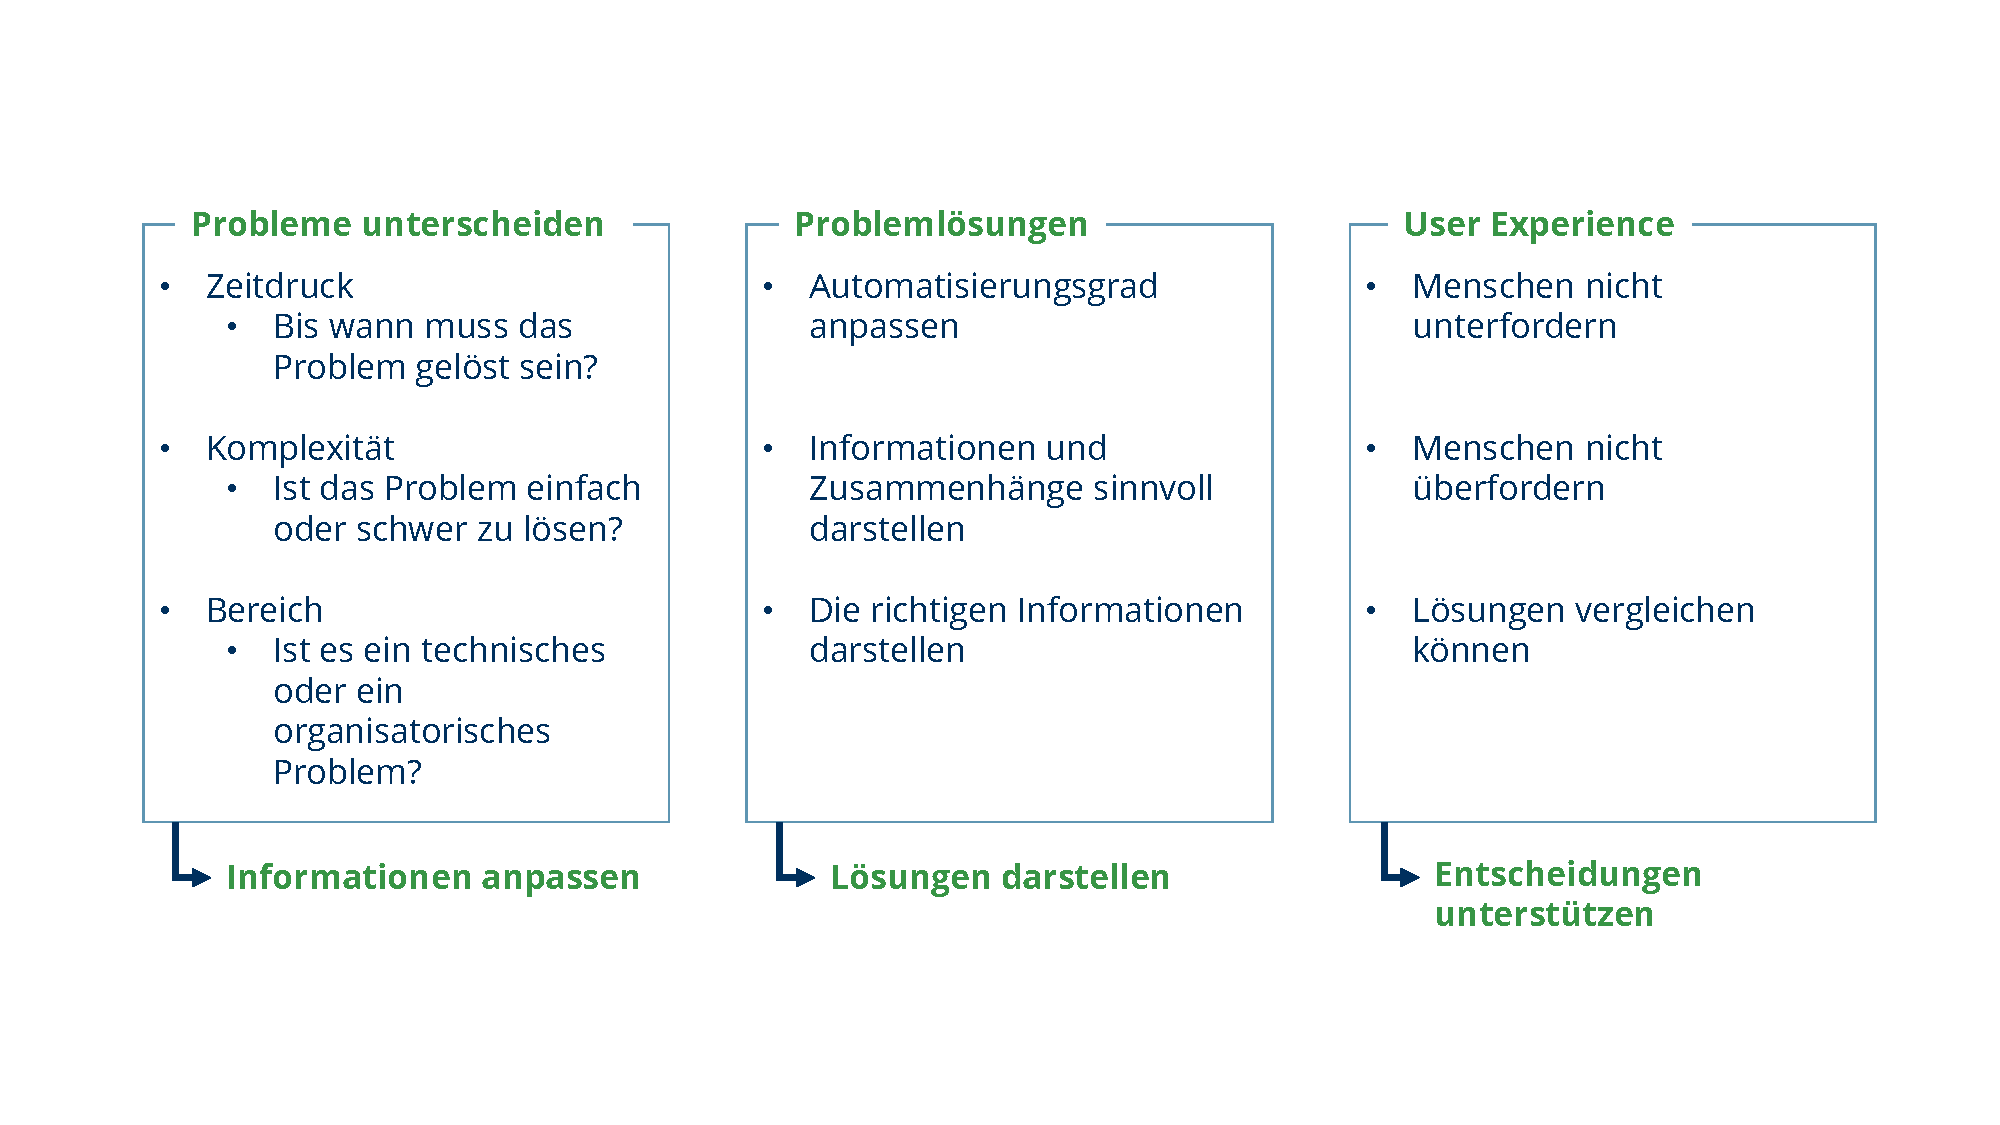
\includegraphics[scale=0.45]{DA_files/Bilder/Konzept/Nutzer-unterstuetzen.pdf}
\caption{•}
\label{pic:Nutzer-Unterstuetzen}
\end{figure}
\\ \\
In Abschnitt \ref{2:Unterscheidung-Probleme} ist bereits aufgeführt, dass sich \textbf{Probleme unterscheiden}. Die Informationen sollen sich entsprechend dem Zeitdruck, der Komplexität des Problems und dem umfassenden Bereich automatisch anpassen. Dadurch soll sowohl eine Unterforderung, als auch eine Überforderung des Menschen verhindert werden.

Die \textbf{Lösungen für das Problem} sollen sinnvoll dargestellt werden. Dabei wird der Autonomiegrad anhand des Zeitdrucks angepasst. Die Menge an dargestellten Informationen und deren Zusammenhänge orientieren sich an der Komplexität des Problems. Die Komplexität des Problems lässt sich aus der Menge an Zusammenhängen ableiten. Deshalb ist es umso wichtiger diese strukturiert und klar darzustellen. Abhängig vom Bereich des Problems sind die richtigen Informationen darzustellen.

Mit einer guten \textbf{User Experience} soll die Entscheidung des Menschen unterstützt werden. Dieser soll mittels geeignetem Autonomiegrad nicht unterfordert werden. Durch die angemessene Darstellung der Informationen ist eine Überforderung zu vermeiden. Die Darstellung der Informationen hängt auch mit der Vergleichbarkeit der Lösungen zusammen. Gibt es mehrere Lösungen, so muss der Nutzer Unterschiede gut erkennen können, um eine geeignete Entscheidung zu treffen.
\\ \\
Wie kann nun der Nutzer durch den Problemlöseprozess begleitet werden? In Abschnitt \ref{2:Phasen-Problemloesen} sind die Phasen des Problemlösens beschrieben. Angelehnt daran wird folgender Ablauf mit entsprechender Unterstützung durch das Assistenzsystem vorgesehen (siehe Bild \ref{pic:Konzeptidee}).
\begin{figure}[htbp]
\centering
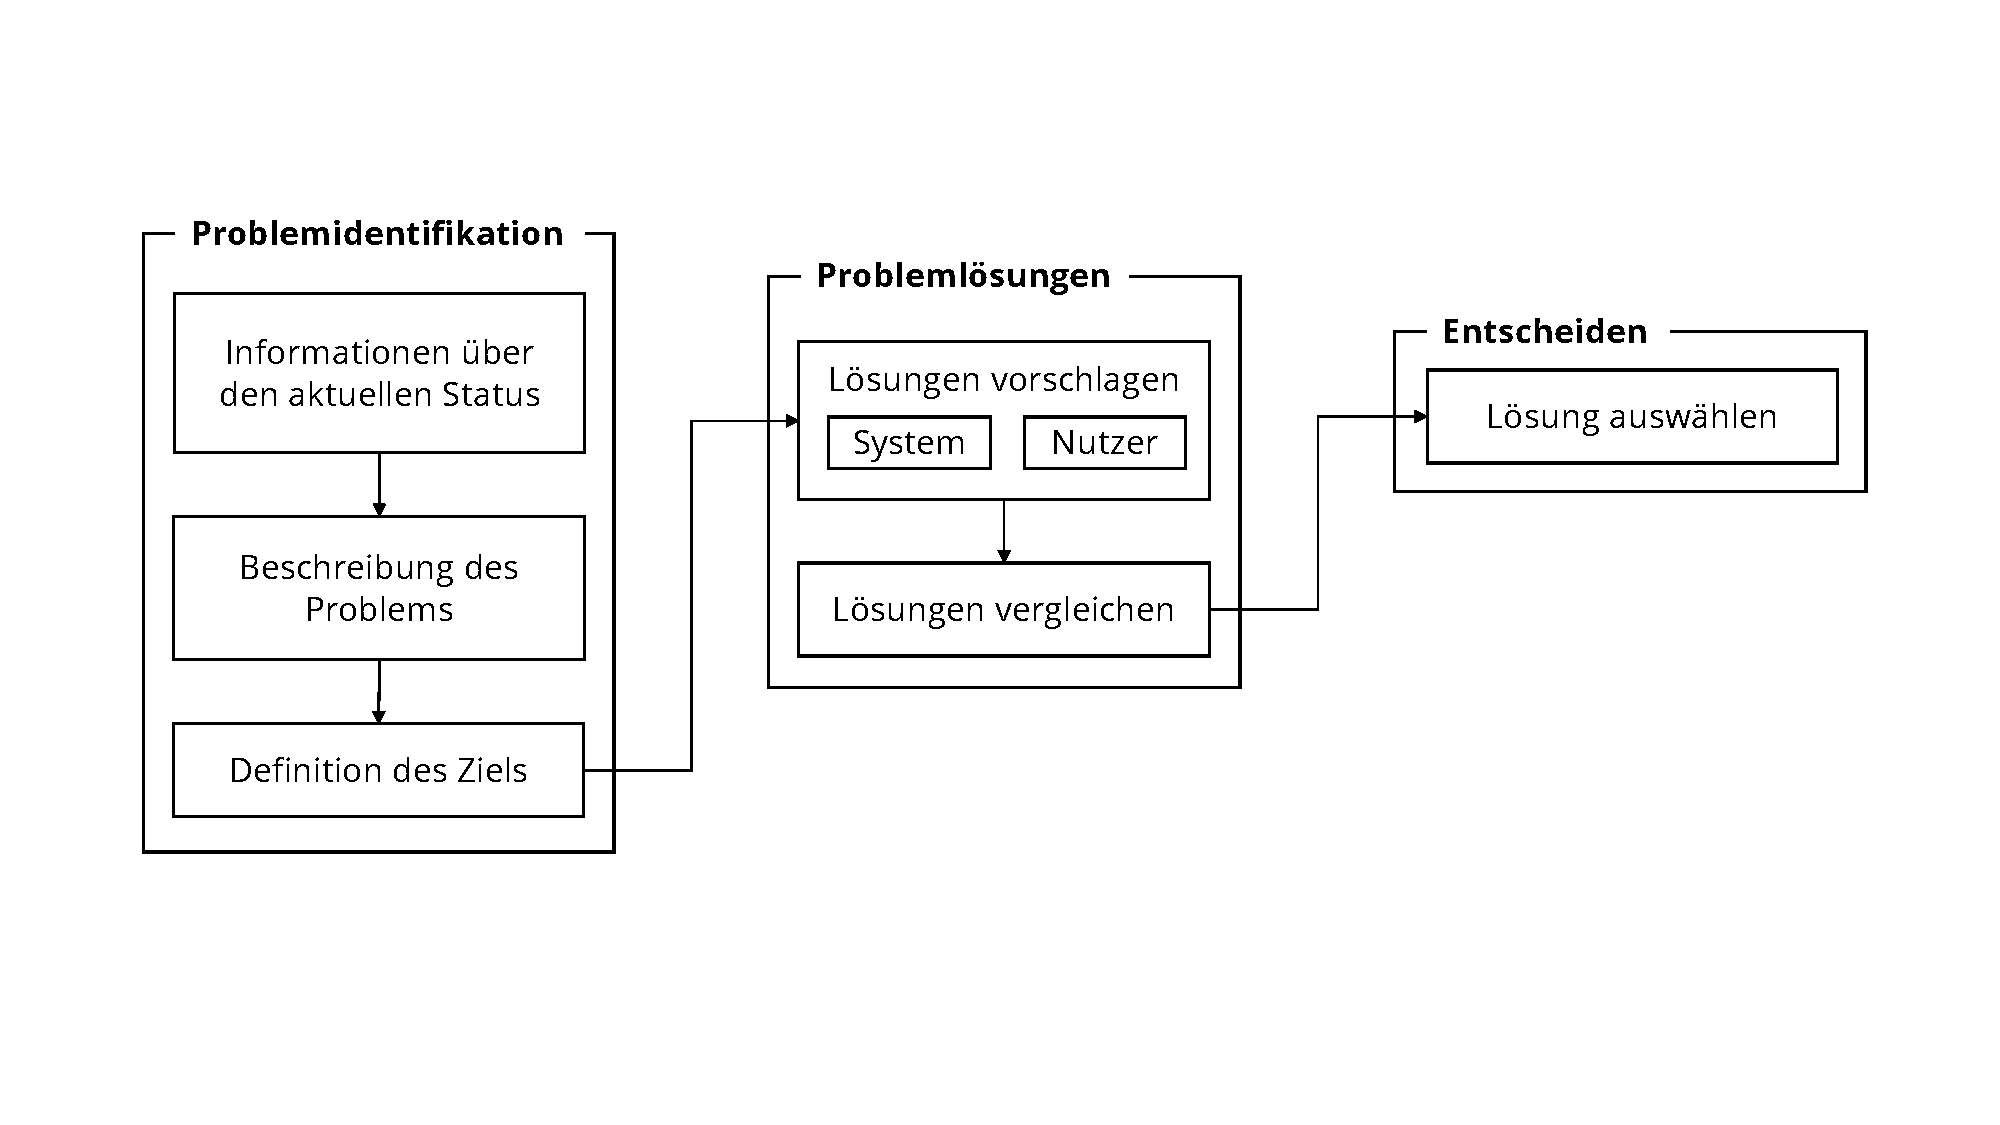
\includegraphics[scale=0.45]{DA_files/Bilder/Konzept/Konzeptidee.pdf}
\caption{Die Schritte des Problemlöseprozess}
\label{pic:Konzeptidee}
\end{figure}

Zunächst muss das Problem identifiziert werden. Dazu stehen dem Nutzer alle Informationen über den aktuellen Status der modularen Anlage zur Verfügung. Dadurch kann der Nutzer einerseits selber Probleme definieren, wie \glqq Das Modul muss nächste Woche gewartet werden. Ein Produktionsausfall ist zu vermeiden.\grqq Andererseits können Probleme auch durch das System identifiziert werden, wenn ein Modul eine Warnung oder einen Alarm auslöst. Ist das Problem identifiziert, so muss das Ziel definiert werden. So kann im Fall des zu wartenden Moduls ein maximaler Produktionsausfall und die dadurch entstehenden Kosten angegeben werden.

Ist das Problem identifiziert und das Ziel definiert, so müssen die möglichen Lösungen betrachtet werden. Lösungen können sowohl vom System als auch vom Nutzer vorgeschlagen werden. Nach Bestimmung der Lösungen erfolgt ein Vergleich dieser. Um eine Entscheidung treffen zu können ist eine Bewertung der verschiedenen Lösungen möglich.

Die Entscheidung wird unterstützt, indem sich die Kriterien und deren Relevanz festlegen lassen. Anhand dieser können die Lösungen gefiltert und die Beste ausgewählt werden.

\subsection{Funktionen}


welche Funktionen müssen realisiert werden?

welche Elemente beeinflussen sich gegenseitig?

\section{Physikalisches Design}